\section{Mixture Models}


\begin{frame} 
\mode<presentation>{
    \begin{center} \huge
        \secname
    \end{center}
    }
    \begin{center} \large
        A class of models that can cluster the data and keep track of importance by estimating densities around clusters.
    \end{center}
	
\end{frame}

\subsection{Many ways of describing the same thing}

\begin{frame}{\subsecname}

Mixture Models\ldots
\begin{itemize}
\item combine density estimation and clustering
\item cluster the data and estimate the density around each cluster
\item increase the resolution of your density estimation in order to end up with a mode around each cluster of data
\item Assume $M$ source are generating points in the data. Find a measure for:
	\begin{enumerate}
	\item the probability of a source $\{q_1,q_2,\ldots,q_M\}$ generating \emph{any} point (How much are you contributing to the data?)
	\item the probability of a point coming from source $q_1$ vs. $q_2$ vs. \ldots vs. $q_M$. Who generated this point?
	\end{enumerate}
\end{itemize}

\end{frame}

\begin{frame}{Model class}

Let $\vec x \in \R^N \sim P(\vec x)$ (data generating distribution)

The Mixture Model breaks down the data generating distribution $P(\vec x)$ into\notesonly{ a linear combination as follows}:

\begin{equation}
	P_{(\vec{x})} = \sum_{q=1}^{M} P_{(\vec{x} | q)} P_{(q)}
\end{equation}
	
$P_{(\vec{x} | q)}:$ components: probability density, that data point $\vec{x}$ was created by component $q$.
\\\vspace{0.3cm}
$P_{(q)}:$ mixture parameters: probability, that component $q$ creates a data point. (How much are you contributing to the data?)

\end{frame}

\subsection{Gaussian Mixture Models}

\definecolor{darkgreen}{rgb}{0,0.6,0}

\begin{frame} 
\only<1,2,3>{
\mode<presentation>{
    \begin{center} \huge
        \subsecname
    \end{center}
    }
    
\pause
    
    \begin{center} \large
        Mixture Model with Gaussians (parametric) as choice of basis function:
        \begin{equation}
        P(x|q) \sim \mathcal{N}(\vec \mu_q, \overbrace{\sigma^2_q \vec I}^{=: \vec \Sigma})
        \end{equation}
    \end{center}
}

\pause

\begin{center}
	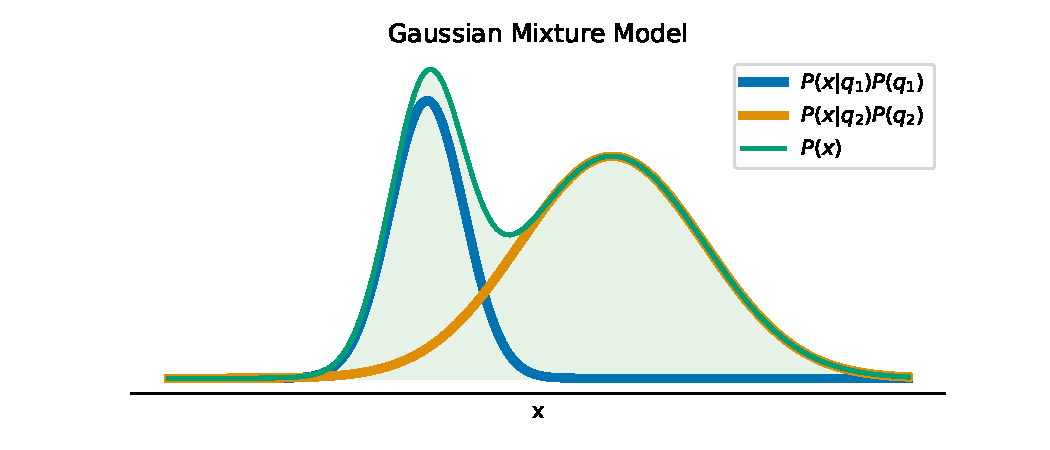
\includegraphics[width=0.7\textwidth]{img/gmm}
	\notesonly{\captionof{figure}{Example Mixture Model with 2 Gaussian components}}
	\label{fig:gmmexample}
\end{center}

\pause

\notesonly{
The density in \figref{fig:gmmexample} can be formulated using:
}

\svspace{-11mm}

\begin{align}
{\color{darkgreen}P(x)} &= {\color{blue}P(x|q_1)~P_{(q_1)}} + {\color{orange}P(x|q_2)~P_{(q_2)}}\\
&= {\color{blue}\mathcal{N}(\mu_1, \sigma^2_1)~\frac{1}{3}} + {\color{orange}\mathcal{N}(\mu_2, \sigma^2_1)~\frac{2}{3}}
\end{align}

\pause

Find estimates for the parameters by maximizing the log-likelihood. This is equivalent to\notesonly{ minimizing the negative log-likelihood w.r.t. to those parameters:}

\svspace{-7mm}

\begin{align}
E^T = - \ln P_{\left( \left\{ \vec{x}^{(\alpha)} \right\} \right)} &= - \sum_{\alpha=1}^{p} \ln \sum_{q=1}^{M} P_{(\vec{x}^{(\alpha)} | q)} P_{(q)} \eqexcl \min_{\text{parameters}}\\
&= - {\color{blue}\mathcal{N}(\mu_1, \sigma^2_1)~P_{(q_1)}} + {\color{orange}\mathcal{N}(\mu_2, \sigma^2_1)~P_{(q_2)}}
\eqexcl
\kern-2ex
\min_{\substack{
\mu_1,~\sigma^2_1,~\mu_2,~\sigma^2_2,\\ P_{(q_1)},~P_{(q_2)}}}
\end{align}

\end{frame}

\subsection{Relation to soft-clustering}

\mode<presentation>{
\begin{frame}
\begin{center}
	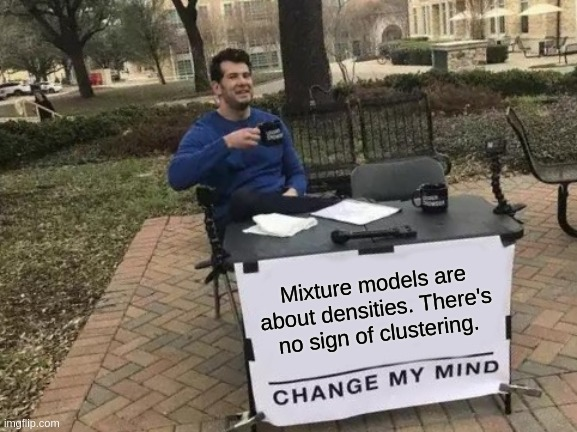
\includegraphics[width=0.5\textwidth]{img/meme_gmmclustering}
\end{center}
\end{frame}
}

\begin{frame}{\subsecname}

\question{How do you get a Gaussian mixture model to act as soft K-means?}

\pause

- We construct the Gaussian Mixture Model using the following assumptions:
\begin{itemize}
	\item Gaussian mixture model with $M$ components
	\item same widths $\sigma_q^2 = \sigma^2 \coloneqq \underbrace{\frac{1}{\beta}}_{\text{given}}$ for all basis functions
	\item same mixture parameters $P_{(q)} = \frac{1}{M}$
\end{itemize}

\end{frame}

\begin{frame}{\subsecname}

For $M$ clusters/components:\\
Let $\vec x^{(\alpha)} \in \R^N$ with $\alpha = 1,\ldots,p$ and $q = 1,\ldots,M$.

% Please add the following required packages to your document preamble:
% \usepackage{graphicx}
\begin{table}[]
\centering
\resizebox{\textwidth}{!}{%
\begin{tabular}{cc|c}
                               & \multicolumn{1}{c|}{soft K-means} & \multicolumn{1}{c}{Gaussian Mixture Models} \\ \cline{2-3} 
\begin{tabular}[c]{@{}c@{}}assignment\\ probabilities\end{tabular}       & $ \big< m_q^{(\alpha)} \big>_Q = \frac{ \exp \big\{ -\frac{\beta}{2}
	\big( \vec{x}^{(\alpha)} - \vec{w}_q^{\mathrm{old}} \big)^2 \big\} }{
	\sum\limits_r \exp \big\{ -\frac{\beta}{2}
	\big( \vec{x}^{(\alpha)} - \vec{w}_r^{\mathrm{old}} \big)^2 \big\}}
	\hspace{0.1cm} \quad \forall \hspace{0.1cm} \alpha, q
$                                  &  
$
P_{(q | \vec{x})} = \frac{\exp \left\{ - \frac{\beta}{2} \left( \vec{x} - \vec{w}_q \right)^2 \right\}}{ \sum_{\gamma=1}^{M} \exp \left\{ - \frac{\beta}{2} \left( \vec{x} - \vec{w}_{\gamma} \right)^2 \right\}}
$                                           \\ \cline{2-3} 
\multicolumn{1}{l}{prototypes} &  $ \vec{w}_q^{\mathrm{new}} \hspace{0.2cm}= \frac{\sum\limits_{\alpha} \big< 
	m_q^{(\alpha)} \big>_Q \vec{x}^{(\alpha)} }{
		\sum\limits_{\alpha} \big< m_q^{(\alpha)} \big>_Q}
		\hspace{0.1cm} \quad \forall \hspace{0.1cm} q
$                                 &   
$\vec{w}_r = \frac{\sum_{\alpha=1}^{p} P_{(r | \vec{x}^{(\alpha)})} \vec{x}^{(\alpha)}}{\sum_{\alpha=1}^{p} P_{(r | \vec{x}^{(\alpha)})}}$                                        \\ \cline{2-3} 
\end{tabular}%
}
\end{table}

\pause

\question{Where did these quantities for GMMs come from?}

\end{frame}

\begin{frame}{\subsecname}


Likelihood of a single sample $\vec x^{(\alpha)} \in \R^N$:
\begin{align}
P_{(\vec{x}^{(\alpha)})} &= \sum_{q=1}^{M} \mathcal{N}\left( \vec{x}^{(\alpha)}; \vec{w}_q, \sigma_q^2 \right) P_{(q)} \\
&= \frac{1}{M}\left(\frac{\beta}{2\pi}\right)^{N/2} \sum_{q=1}^{M} \exp \left\{ - \frac{\beta}{2} \left( \vec{x}^{(\alpha)} - \vec{w}_q \right)^2 \right\} 
\end{align}

Minimizing the cost w.r.t. to the parameters by minimizing the negative data log-likelihood:

\vspace{-2mm}

\begin{align}
E^T = - \ln P_{\left( {\color{red}\left\{ \vec{x}^{(\alpha)} \right\}} \right)} &= -\ln {\color{red}\prod_{\alpha=1}^{p}}
\bigg\{ \sum_{q=1}^{M} \mathcal{N}\left( \vec{x}^{(\alpha)}; \vec{w}_q, \sigma_q^2 \right) P_{(q)}
\bigg\} 
\\&= - {\color{red}\sum_{\alpha=1}^{p}} \ln \sum_{q=1}^{M} \exp \left\{ - \frac{\beta}{2} \left( \vec{x} - \vec{w}_q \right)^2 \right\} + \text{const}_{(q)}
\end{align}

\end{frame}

\begin{frame}{\subsecname}

The prototypes are found by estimating the means of the individual components.

We compute the derivative of the cost w.r.t an individual prototype $\vec w_r$, set it to zero and solve for $\vec w_r$:

\begin{align}
\frac{\partial E^T}{\partial \vec{w}_r} &= - \sum_{\alpha=1}^{p} \frac{\overbrace{\exp \left\{ - \frac{\beta}{2} \left( \vec{x} - \vec{w}_r \right)^2 \right\}}^{P_{(r|\vec x)}}}{\sum_{q=1}^{M} \exp \left\{ - \frac{\beta}{2} \left( \vec{x} - \vec{w}_q \right)^2 \right\}} \beta \left( \vec{x} - \vec{w}_r \right) \eqexcl \vec 0 \\
\vec{w}_r &= \frac{\sum_{\alpha=1}^{p} P_{(r | \vec{x}^{(\alpha)})} \vec{x}^{(\alpha)}}{\sum_{\alpha=1}^{p} P_{(r | \vec{x}^{(\alpha)})}} \quad \leadsto \substack{\text{ center of mass condition}\\\text{for soft-clustering!}}
\end{align}

\end{frame}

\begin{frame}{\subsecname}

\question{What about the assignment probabilities?}

\svspace{-3mm}

\only<1>{
In soft-clustering we have the assignment probabilities $m_q^{(\alpha)} \in \lbrack 0,1 \rbrack$ to reflect the probability of a point $\vec x^{(\alpha)}$ being assigned to cluster $q$ with $\sum_{q=1}^M m_q^{(\alpha)} = 1$.
}

\only<2,3>{
In Mixture Models we have a probabilistic setting with the following quantities. \only<3>{Adding a Bayesian ``perspective'' to them gives us:}

\begin{itemize}
\item $P_{(\vec x)}$ : likelihood \only<3>{(\emph{prior} of the data)}
\item $P_{(q)}$: the probability of component $q$ creating a point \only<3>{(\emph{prior} of the component) $\leadsto$ constraint $\sum_{q=1}^M P_{(q)} = 1$}
\item $P_{(\vec x|q)}$ : the probability density that a point $\vec x$ was created by component $q$
\end{itemize}
}

\only<3>{

\svspace{-5mm}

\begin{align}
P_{(q | \vec{x})} P_{(\vec{x})} &= P_{(\vec{x} | q)} P_{(q)} \\
P_{(q | \vec{x})} &= \frac{P_{(\vec{x} | q)} P_{(q)}}{P_{(\vec{x})}}
\end{align}

$P_{(q | \vec{x})}$: posterior probability of component q having generated a given data point $\vec{x}$

}

\only<4>{

$\leadsto$ given the simplified Gaussian mixture model we obtain:
\begin{eqnarray}
P_{(q | \vec{x})} &=& \slidesonly{\frac{P_{(\vec{x} | q)} P_{(q)}}{P_{(\vec{x})}} = } \frac{
\overbrace{\left( \frac{\beta}{2\pi} \right)^{N/2} \exp \left\{ - \frac{\beta}{2} \left( \vec{x} - \vec{w}_q \right)^2 \right\}}^{P_{(\vec x|q)}} \cdot \overbrace{\frac{1}{M}}^{P_{(q)}}}{
\underbrace{\left( \frac{\beta}{2\pi} \right)^{N/2} \frac{1}{M} \sum_{\gamma=1}^M \exp \left\{ - \frac{\beta}{2} \left( \vec{x} - \vec{w}_{\gamma} \right)^2 \right\}}_{
P_{(\vec x)}
}} \\
&=& \frac{\exp \left\{ - \frac{\beta}{2} \left( \vec{x} - \vec{w}_q \right)^2 \right\}}{ \sum_{\gamma=1}^{M} \exp \left\{ - \frac{\beta}{2} \left( \vec{x} - \vec{w}_{\gamma} \right)^2 \right\}}
\end{eqnarray}
}

\end{frame}

\subsection{Remarks}

\begin{frame}{\subsecname: A constraint for the mixture parameters}

\question{Why do we need to constrain the mixture parameters $P_{(q)}$ s.t. they sum up to 1?}

\svspace{-5mm}

\begin{equation}
\sum_{q=1}^M P_{(q)} = 1
\end{equation}

\pause

- To avoid solutions with ``by-standing'' components that don't contribute to the dataset.

Side effect:\\

If $M$ is chosen too large, a solution may contain a component with a very low mixture parameter $P_{(q)}$ that is only useful for explaining a very small portion of the dataset (e.g. a component that explains a single point)

Such ``degenerate'' solutions or ``collapse'' of the mixture model can be avoided by choosing a smaller $M$.

\end{frame}
